\chapter{設計}
\label{chap:sekkei}

本章ではハイパーイラストと手書きベースWikiの要件と設計について述べる。

\newpage

\section{要件}
前章で示した画像ファイルフォーマットや手書きデータを扱う既存のツールの問題点を踏まえて、本システムの要件を整理する。
\begin{enumerate}
    \item 簡単に手書きメモのメモやイラストが作成・編集できる\\
    気軽に手書きメモ・イラストを取ることができ、また再編集性も可能である。
    \item 作成した手書きのメモやイラストを簡単に参照したり、再利用したりできる\\
    画像の内部に対してハイパーリンクを設定でき、関連する画像を参照することができる。
\end{enumerate}
これらの要件を満たすシステムは次世代の画像ファイルフォーマットであるハイパーイラストと、その作成・編集と管理をサポートする手書きベースWikiの組み合わせによって実現可能である。

\section{ハイパーイラスト}
本研究ではハイパーテキストの特徴を取り入れることによって既存の画像ファイルフォーマットの問題点を解決する
ハイパーイラストを提案する。

\subsection{ハイパーイラストの定義}
\begin{itemize}
    \item テキストではなく手書きによって記述される \\
    HTML等のハイパーテキストは記法に基づいたテキストによってマークアップされるが、
    ハイパーイラストはタッチやスタイラスから取得される手書きデータによってその内容が記述される。
    \item 内部の任意の要素にハイパーリンクが埋め込むことができる \\
    ハイパーテキストがその内部に他の文書への参照を示すハイパーリンクを埋め込むことができるように、
    ハイパーイラストは内部にハイパーリンクを埋め込むことができる。
\end{itemize}

\begin{figure}[htbp]
    \begin{center}
    \fbox {
\includegraphics[width=50mm]{images/testimage.png}} \end{center}
    \caption{ハイパーイラストの概念図}
\end{figure}

\subsection{ハイパーイラストの仕様}
本研究におけるハイパーイラストはSVG\cite{aboutsvg}というフォーマットをベースとしている。
SVGはXML\footnote{https://www.w3.org/XML/}をベースとしており、他の画像ファイルフォーマットにはない、ハイパーイラストに適した以下のような特徴を持つ。
\begin{itemize}
    \item グラフィカルな表現を前提に設計されている\\
    SVGには曲線等を表現するPath要素や閉じた図形を表現するPolygon要素等の仕様が標準で備わっている。
    スタイラスから得られるデータをPath要素の属性として定義することで手書きのストロークを表現することができる。
    (例えばソースコード\ref{tegakipathcode}で図\ref{tegakipath}のように表現できる)
    \item 構造を保持できる\\
    ラスターイメージと異なりSVGの実体は構造化されたテキストファイルであり、線分や点はピクセルではなく
    独立した要素として記述される。これにより書き順や編集履歴等の構造も保持され、再編集性が高い。
    \item ハイパーリンクを埋め込める\\
    SVGではXLink\footnote{https://www.w3.org/TR/xlink/}形式のハイパーリンクを任意の要素に埋め込むことができるため
    画像の中の個別の要素に対して複数のリンクを定義することができる。
    \item Web標準の技術である\\
    SVGは特定の企業の製品ではなく、その仕様は全て公開されている。また作成や表示に特別なソフトウェアを必要とせず、
    ブラウザのみで閲覧することができる。
\end{itemize}

\begin{figure}[htbp]
    \begin{center}
        \fbox {
\includegraphics[width=70mm]{images/svgpath.png}} \end{center}
    \caption{SVG上で表現される手書きストローク} \label{tegakipath}
\end{figure}

\begin{lstlisting}[caption=図\ref{tegakipath}の実体, label=tegakipathcode]
    <path stroke-linejoin="round" stroke-linecap="round" stroke="#585858"
    stroke-width="10" class="" pointer-events="auto" fill="rgba(0,0,0,0)"
    id="1072-528" d="M 919 564 ,L 919 563 ,L 919 562 ,L 919 560 ,L 919 559 ... L 1064 520 "></path>
\end{lstlisting}


\section{手書きベースWiki}
%本研究で提案する手書きベースWikiの基本構成及び使い方を解説する。
%既存のテキストベースWikiがテキスト入力によって作成されたハイパーテキストをコンテンツとするように、
%手書きベースWikiでは手書き入力によって作成されたハイパーイラストをコンテンツとして管理する。
ハイパーイラストをコンテンツとするWikiシステムである手書きベースWikiも提案する。


\subsection{手書きベースWikiの定義}
\begin{itemize}
    \item ハイパーイラストを作成・編集できる\\
    タッチやスタイラスに対応したエディタを備え、手書きによって
    ハイパーイラストを手軽に作成・編集することができる。
    \item ハイパーイラストにハイパーリンクを追加できる \\
    作成したハイパーイラスト同士の相互リンクを簡単な操作で定義できる。
    \item 関連するハイパーイラストを参照できる \\
    ハイパーイラスト同士のリンク関係を元に、関連するハイパーイラストを
    推薦し、一覧できるよう表示する。
\end{itemize}
この要件を満たす手書きベースWikiのプロトタイプとしてDrawWikiを開発した。

\subsection{DrawWiki}
DrawWikiは本研究において開発した、手書きベースWikiのコンセプトを元にしたプロトタイプとなるアプリケーションである。(図\ref{drawwiki})
本章ではその主要な機能を使い方とともに解説する。

\begin{figure}[htbp]
    \begin{center}
    {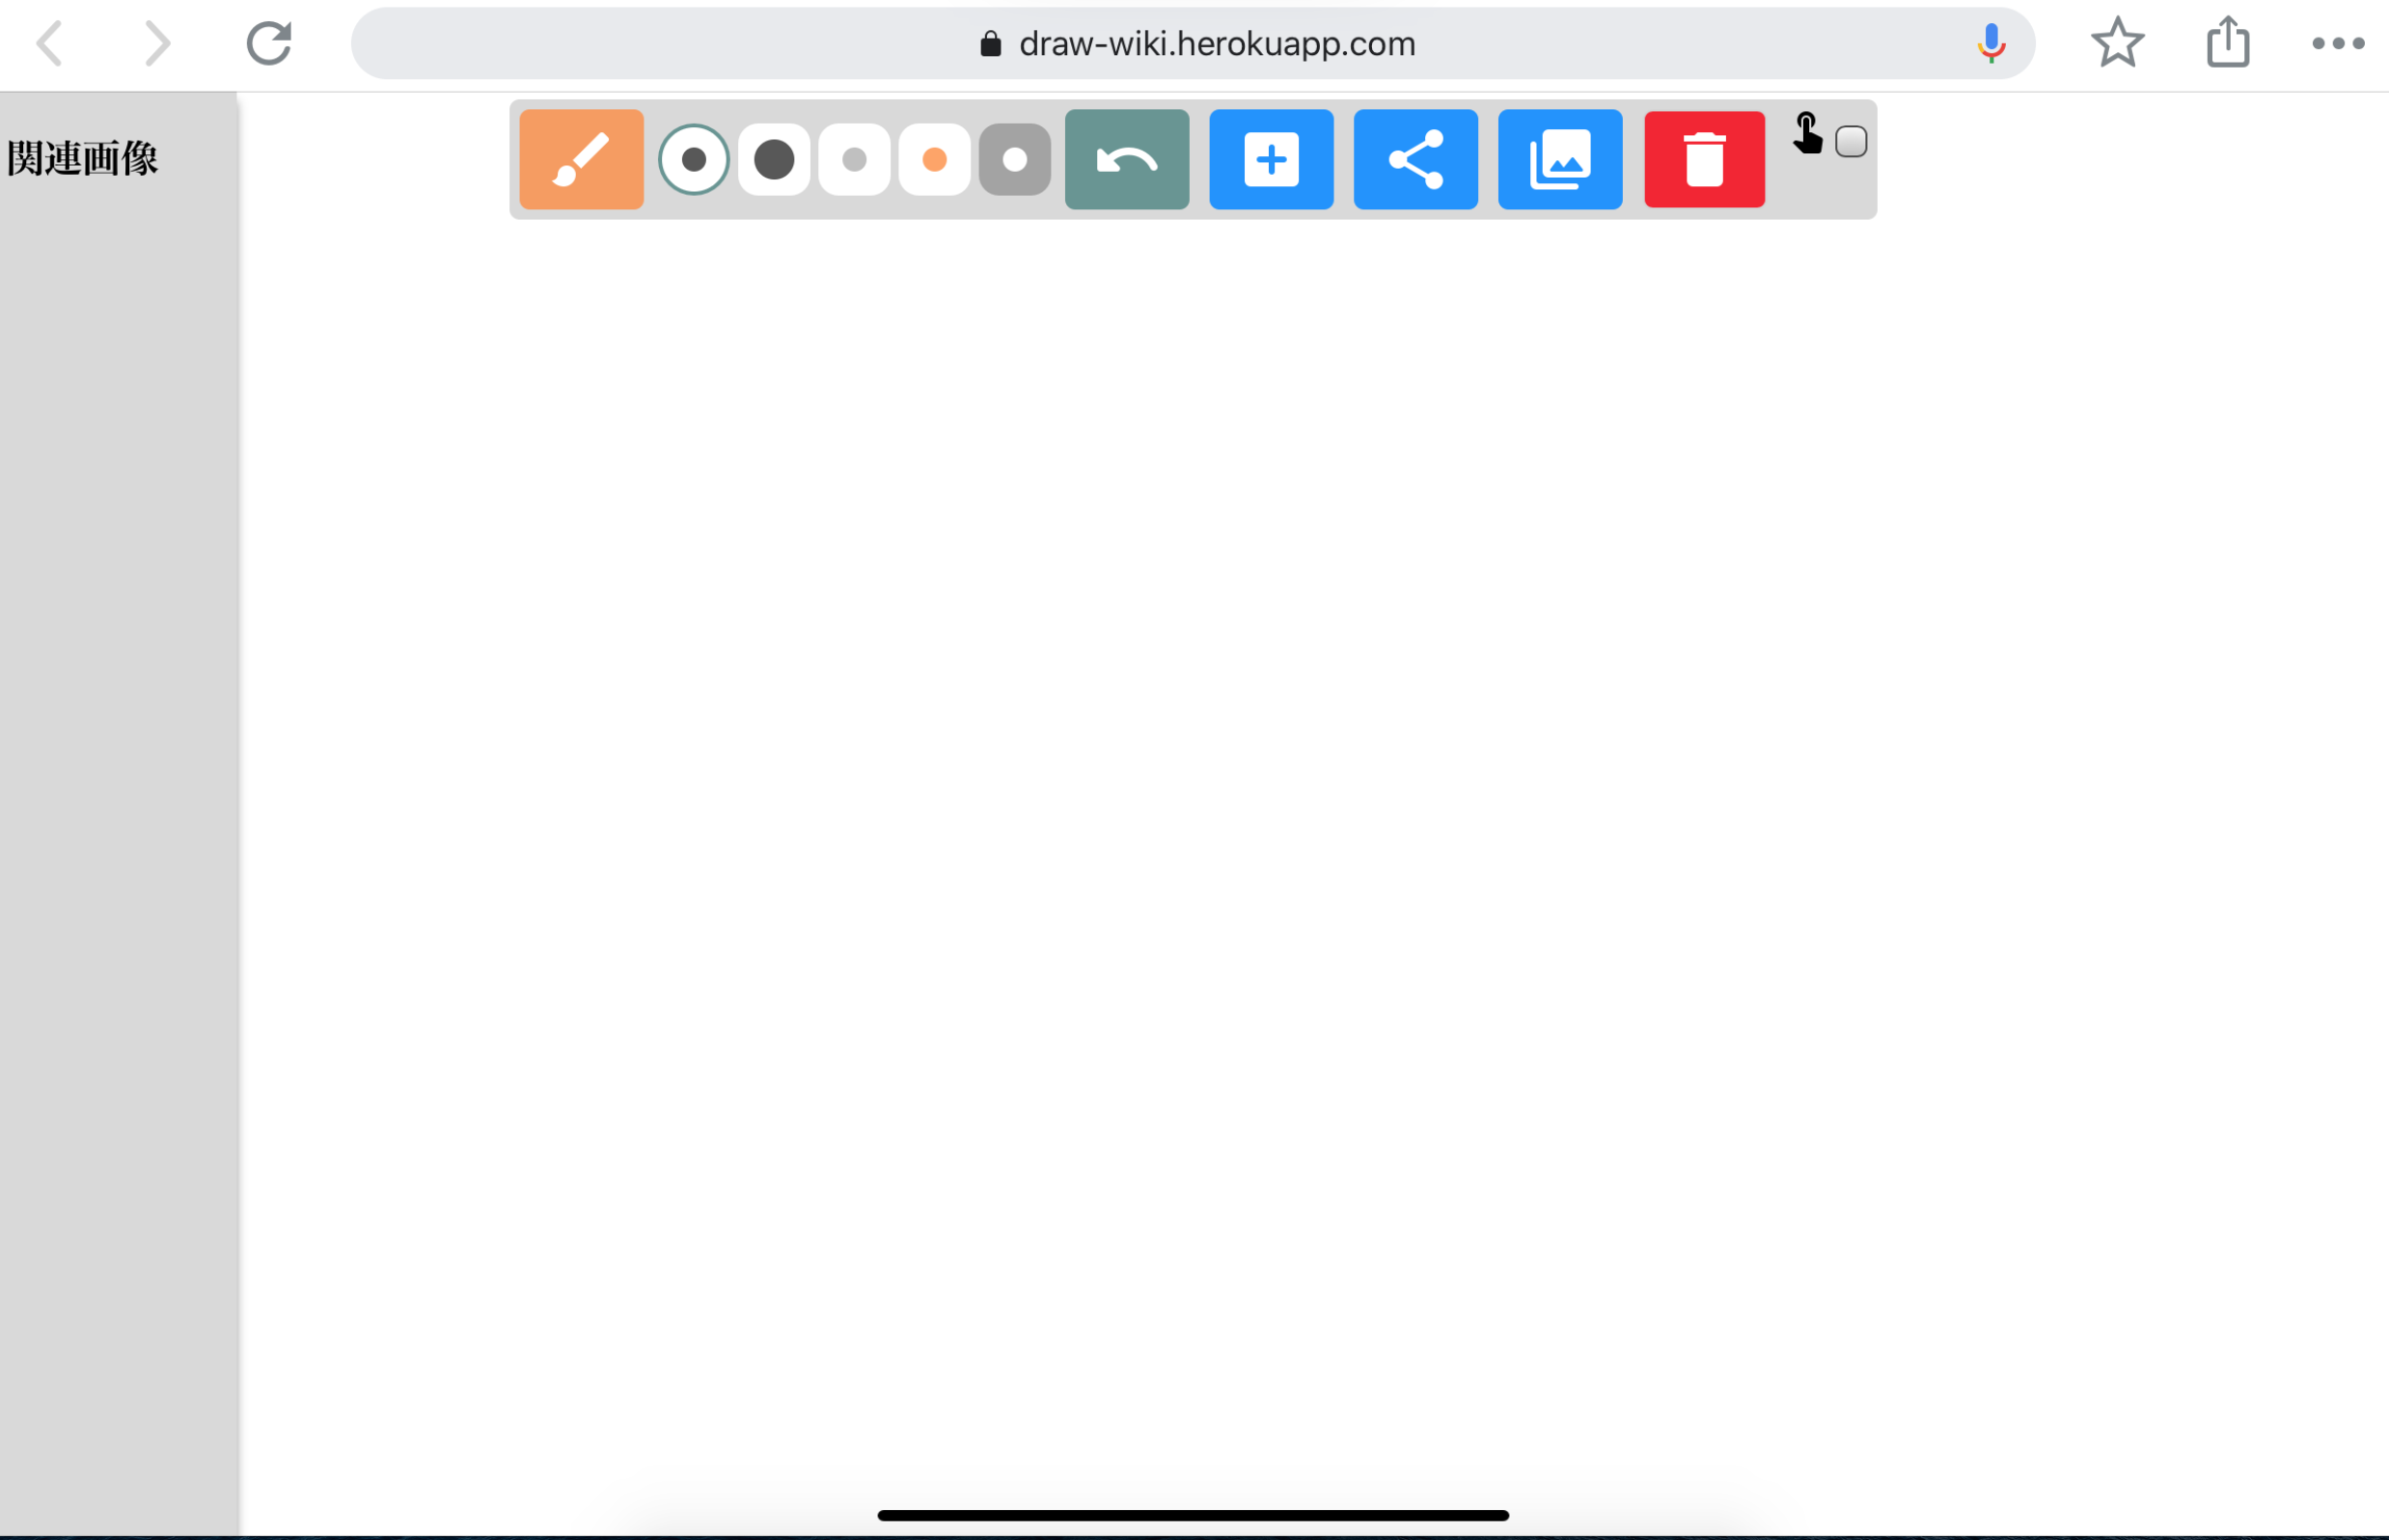
\includegraphics[width=100mm]{images/initialdrawwiki.png}} \end{center}
    \caption{DrawWikiの初期画面}
    \label{drawwiki}
\end{figure}

\subsection{機能と使い方}

\subsubsection{ハイパーイラストの作成・編集}

\begin{figure}[htbp]
    \begin{center}
        \fbox {
\includegraphics[width=100mm]{images/testimage.png}} \end{center}
    \caption{ハイパーイラストの作成画面}
    \label{hyperillustcreate}
\end{figure}

画面中央部分に自由に手書きができるキャンバスが配置されており、ここに描いたものが
ハイパーイラストとして自動的に保存・アップロードされる。
一度アップロードしたハイパーイラストには一意なURLが割り振られるため、
Webを通じて他のユーザーが閲覧し、また編集することもできる。

\subsubsection{ブラシプリセット}
メモやアイデアスケッチ等の用途であればさほど多くのブラシは要求されない。必要以上の機能はソフトウェアの使い方を習得する妨げとなりうるため、
DrawWikiでは金箱らによるInteractive Sketch\cite{130004638060}に基づいたコンパクトなブラシプリセット構成を採用している。
このスケッチ技法は以下の4種類のブラシを用いる
\begin{enumerate}
    \item 通常のペンで全体を描く
    \item 影や質感をグレーで表現する
    \item 輪郭を太い線で縁取る
    \item 特徴的な部分、機能を有する箇所をキーカラーでハイライトする
\end{enumerate}
これによりWikiとして活用する上で有利な以下のような特徴を持つ(図\ref{fig:interactivesketch})。
\begin{itemize}
    \item 太線で図のアウトラインが強調されるためサムネイル状態での視認性が確保される
    \item キーカラーによる強調表示でアイデアが伝わりやすくなる
    \item ブラシによって描き方がある程度統一され、スケッチ技量の巧拙を吸収できる
\end{itemize}

\begin{figure}[htbp]
    \begin{center}
        \fbox {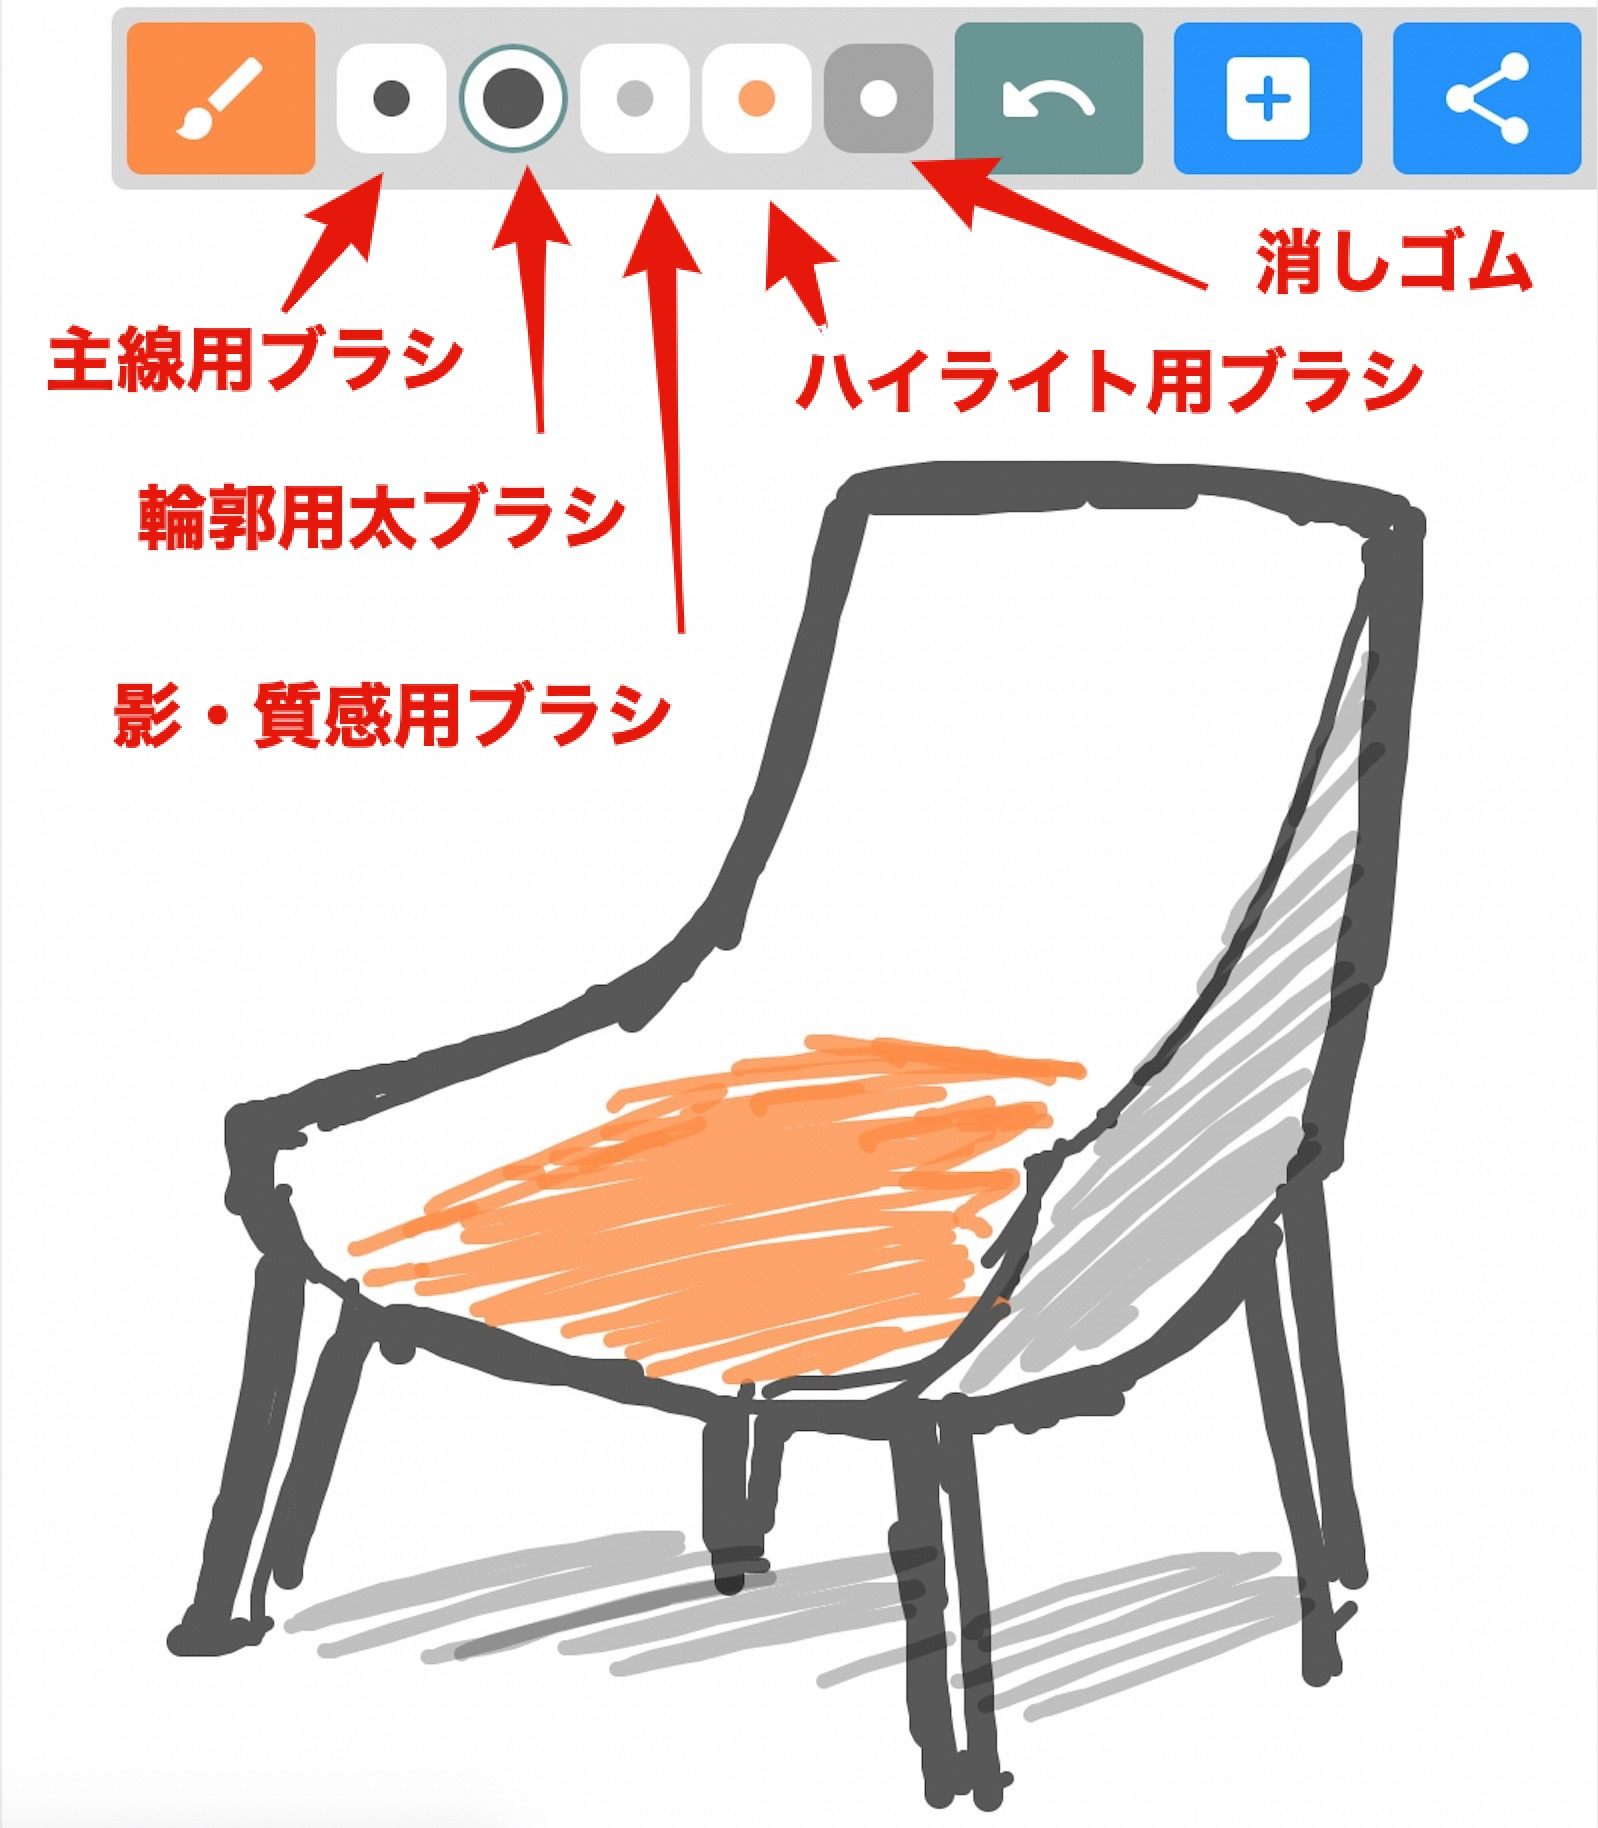
\includegraphics[width=60mm]{images/interactivesketch.jpg}} \end{center}
    \caption{プリセットを用いて描かれた図}
    \label{fig:interactivesketch}
\end{figure}

\subsubsection{ハイパーリンク埋め込み機能}

\begin{figure}[H] \begin{minipage}{0.5\hsize}
                         \begin{center} \fbox {
\includegraphics[width=70mm]{images/testimage.png}}
                         \end{center} \caption{範囲選択ツール} \label{fig:addLink1}
\end{minipage} \begin{minipage}{0.5\hsize}
                   \begin{center} \fbox {
\includegraphics[width=70mm]{images/testimage.png}}
                   \end{center} \caption{リンク埋め込み機能の操作画面} \label{fig:addLink2}
\end{minipage}
\end{figure}

範囲選択ツールを用いてハイパーリンクを埋め込みたい要素を選択することができる。
要素を選択して"他の図とリンクボタン"を押すと今まで作成したハイパーイラストのリストが開き、
その中からリンクさせたい図を選ぶとその図へのハイパーリンクが要素に埋め込まれる。

\subsubsection{関連するハイパーイラストの表示機能}

\begin{figure}[htbp] \begin{minipage}{0.5\hsize}
                         \begin{center} \fbox {
\includegraphics[width=70mm]{images/testimage.png}}
                         \end{center} \caption{関連イラストの表示機能} \label{fig:linkedIllust1}
\end{minipage} \begin{minipage}{0.5\hsize}
                   \begin{center} \fbox {
\includegraphics[width=70mm]{images/testimage.png}}
                   \end{center} \caption{関連イラストのモーダル} \label{fig:linkedIllust2}
\end{minipage}
\end{figure}

エディタの横に位置する"関連画像ビュー"には、
\begin{itemize}
    \item 別のハイパーイラストへのリンク
    \item 別のハイパーイラストからのリンク
%    \item リンク先ハイパーイラストがリンクしているハイパーイラスト
\end{itemize}等のリンクに基づいた関連イラストのサムネイルが表示される(図\ref{fig:linkedIllust1})。
またサムネイルを選択すると、当該ハイパーイラストがリンクしているハイパーイラストをリストするダイアログが表示される(図\ref{fig:linkedIllust2})。
このようにリンクに基づいて関連するイラストを表示し、参照可能にする仕組みが備わっている。

%また、この時ハイパーリンクが埋め込まれている要素が強調表示され、対応関係が理解できるように

%\subsubsection{ハイパーイラストのインポート機能}
%
%\begin{figure}[htbp]
%    \begin{center}
%    {
\includegraphics[width=50mm]{images/testimage.png}} \end{center}
%    \caption{インポート機能の操作画面}
%    \label{importing}
%\end{figure}
%
%過去に作成したハイパーイラストを一覧画面から選択し、現在編集中の画面にインポートすることができる。
%インポートした画像にも、元の画像へのハイパーリンクが含まれている。

\subsubsection{エキスポート・共有機能}

%\begin{figure}[htbp]
%    \begin{center}
%    {
\includegraphics[width=50mm]{images/testimage.png}} \end{center}
%    \caption{エキスポート機能の操作画面}
%    \label{exporting}
%\end{figure}

\begin{figure}[htbp] \begin{minipage}{0.5\hsize}
                         \begin{center} \fbox {
\includegraphics[width=70mm]{images/testimage.png}}
                         \end{center} \caption{エキスポート機能の操作画面} \label{fig:exporting1}
\end{minipage} \begin{minipage}{0.5\hsize}
                   \begin{center} \fbox {
\includegraphics[width=70mm]{images/testimage.png}}
                   \end{center} \caption{埋め込まれたハイパーイラスト} \label{fig:exporting2}
\end{minipage}
\end{figure}
エキスポート機能を利用すると、ハイパーイラスト単体(SVGファイル)のURLを取得することができる。
このSVGのURLはimg要素\footnote{https://developer.mozilla.org/ja/docs/Web/HTML/Element/img}や
Object要素\footnote{https://developer.mozilla.org/ja/docs/Web/HTML/Element/object}等のソースとして指定することが可能で、
図\ref{fig:exporting2}のように他のWebサイトにも埋めこむことができる。